%%%%%%%%%%%%%%%%%%%%%%%%
%
% $Author: Deepti Hegde $
% $Datum: 2023-05-02  $
% $Pfad: BA23-02-Sales-Predictor/report/Contents/en/Packages.tex $
% $Version: 1.0 $
% $Reviewed by: Deepti, Sadegh and Raunak $
% $Review Date: 2023-06-30 $
%
%%%%%%%%%%%%%%%%%%%%%%%%


\chapter{Test Functions}
	
	The test functions behave to confirm the data's integrity and evaluate the prediction model's performance. They provide useful feedback on the data reading process, missing values, and model accuracy, which aids in the detection and resolution of potential code errors.
	In our code, we have 3 main test functions. Namely, test\_csv\_read, test\_missing\_values, and test\_prediction\_function. These are encapsulated within a class named TestDataValidation. The class allows you to organize related functions and variables together.
	
	The class encapsulates related functionality within a single unit, allowing for better organization, code reusability, and easier maintenance. It provides a structured approach to perform data validation tests and ensures that the code meets the expected criteria. 
	To run the tests, an instance of the TestDataValidation class is created (data\_validation = TestDataValidation()), and then the run\_tests method is called (data\_validation.run\_tests()).
	
	\section{Automation }
	
		\begin{itemize}
			
		\item Reading CSV files: 
		
		The code reads multiple CSV files using pandas' read\_csv() function. This automates the process of loading data from CSV files into DataFrames.
		
		\item Data Validation Tests:
		
		The code includes a class named TestDataValidation that performs data validation tests. These tests check for the presence of data in the loaded DataFrames and the presence of expected columns. By running the run\_tests() method, the tests are executed automatically, and any failures or issues are reported.
		
		\item Model Evaluation: 
		
		The code calculates evaluation metrics such as R2 score and mean squared error (MSE) for the predicted values. This automates the process of evaluating the model's performance using pre-defined metrics.
		
		
		\item Test automation: 
		
		Integrating the data validation tests with a testing framework like pytest to automate the execution of tests and generate detailed test reports.
		
		\end{itemize}

	By automating these tasks, the overall workflow can be streamlined, reducing manual effort and potential errors, and enabling efficient and reproducible data analysis and model building.
	
	\section{Test functions used in the project}
	
		\begin{enumerate}
			
			\item \textbf{test\_csv\_read:}
			
			This test function verifies that the CSV files required for analysis are successfully read and that the 'train.csv' file contains the necessary columns. Ensure that the CSV files exist in the specified locations and that the 'train.csv' file has the correct column structure.
			
			\begin{itemize}
				
				\item \textbf{Steps}
				
					\begin{enumerate}
						
						\item Assert that the DataFrames stores, items, trans, oil, holidays, sales and inputdf are not empty, indicating that the corresponding CSV files have been read successfully.
				
						\item Assert that the 'train.csv' DataFrame (sales) contains the expected columns: 'id', 'date', 'store\_nbr', 'item\_nbr', 'unit\_sales', and 'onpromotion'.
						
						\item Assert that the 'input.csv' DataFrame (inputdfTestRead) contains the expected columns: 'id', 'date', 'store\_nbr', 'item\_nbr', and 'onpromotion'.
						
			\end{enumerate}
				
				\item \textbf{Possible Errors and Resolutions:}
				
				\begin{itemize}
					
					\item Error: Failed to read 'stores.csv'
					
					\item Explanation: The 'stores.csv' file could not be read. If there is no record in any of the mentioned csv files, it will through an error.
					
					\item Resolution: Make sure the 'stores.csv' file exists in the specified location and that it is accessible.
					
				\end{itemize}
				
			\end{itemize}
		
			\begin{center}
				\begin{figure}[h!]
					\begin{center}
						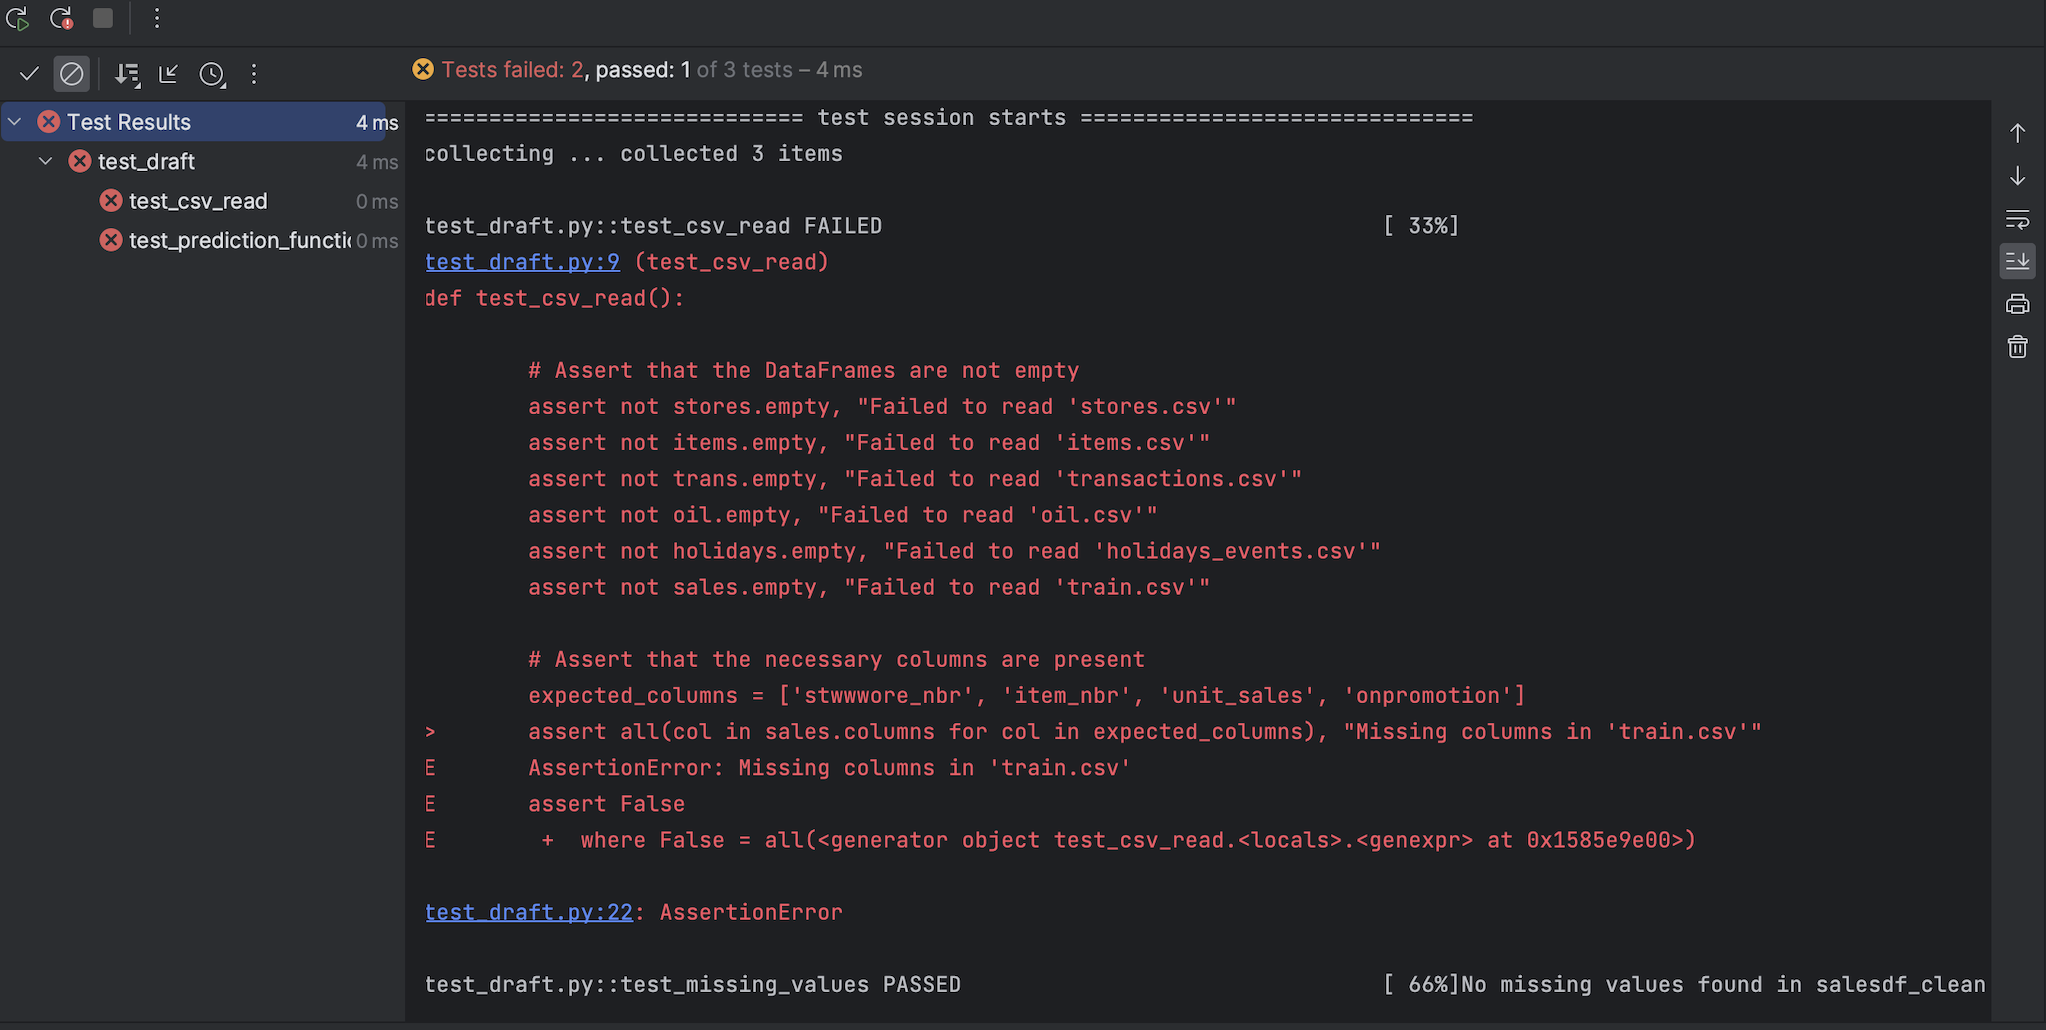
\includegraphics[height=125mm, width=130mm]{Images/TesrCSVResd}
					\end{center}
					\caption{ Possible Error for Test CSV Read Function }
				\end{figure}
			\end{center}
			
			\item \textbf{test\_missing\_values:}
			
			This test function checks if the DataFrame salesdf\_clean contains any missing values (NaN or NA). If missing values are detected in the salesdf\_clean DataFrame, an error will be raised. Handle missing values by imputing or removing them as appropriate for the analysis.
			
			\begin{itemize}
				
				\item \textbf{Steps}
					
					\begin{enumerate}
						
						\item Check for missing values in the salesdf\_clean DataFrame using the isnull().values.any() function.
					
						\item Assert that there are no missing values in salesdf\_clean.
						
						\item Assert that there are no missing values in inputdfTest.
												
				\end{enumerate}
				
				\item \textbf{Possible Errors and Resolutions:}
				
				\begin{itemize}
					
					\item Error: salesdf\_clean contains missing values (NaN or NA)
					
					\item Explanation: The DataFrame salesdf\_clean contains one or more missing values.
					
					\item Resolution: Examine the salesdf\_clean DataFrame and handle any missing values appropriately, such as imputing or removing them.
					
				\end{itemize}
				
			\end{itemize}
		
			\begin{center}
				\begin{figure}[h!]
					\begin{center}
						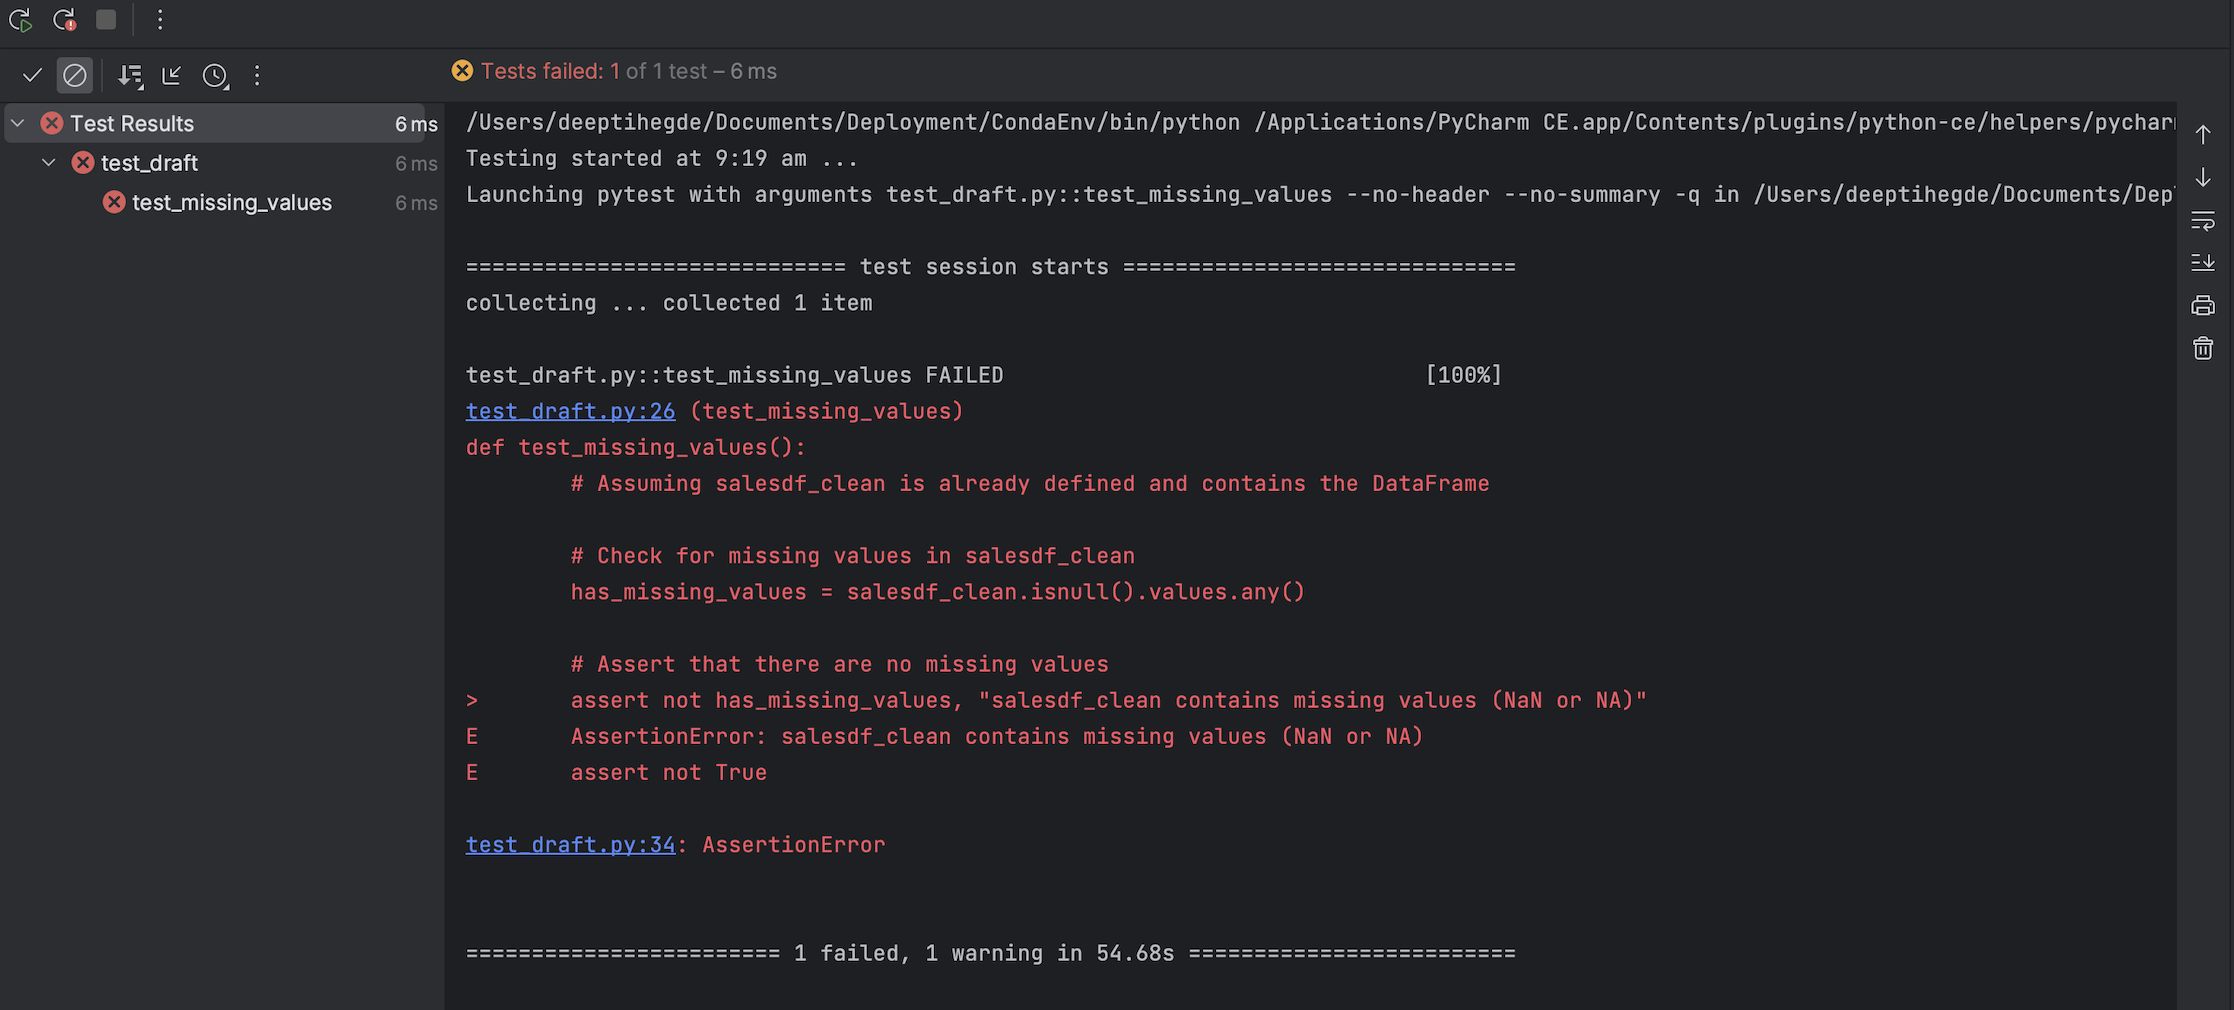
\includegraphics[height=125mm, width=130mm]{Images/TestmsValues}
					\end{center}
					\caption{ Possible Error for Test Missing Values Function }
				\end{figure}
			\end{center}
		
		
			\item \textbf{test\_prediction\_function:}
			
			This test function evaluates the performance of a prediction model by calculating the R-squared (r2) score and mean squared error (mse) between the predicted values (y\_pred) and the true values (y\_test). If the calculated r2 or mse score deviates significantly from the expected values, an error will be raised. Review the model and the evaluation process to identify potential issues that may affect the performance metrics. Adjust the model or evaluation process accordingly.
			
				\begin{itemize}
				
				\item \textbf{Steps}
				
					\begin{enumerate}
						
						\item Calculate the r2 score using the r2\_score() function from the sklearn.metrics module.
						
						\item Calculate the mse score using the mean\_squared\_error() function from the sklearn.metrics module.
						
						\item Assert that the calculated r2 score is approximately equal to the expected value of 0.8 with a tolerance of 0.15. 
						
						\item Assert that the calculated mse score is approximately equal to the expected value of 0.00037 with a tolerance of 0.0001.
					\end{enumerate}
					
				
				\item \textbf{Possible Errors and Resolutions:}
				
				\begin{itemize}
					
					\item Error: The r2 score does not match the expected value within the specified tolerance.
					
					\item Explanation: The calculated r2 score is significantly different from the expected value.
					
					\item Resolution: Review the model and the evaluation process to identify any issues that could affect the r2 score. Adjust the model or evaluation process accordingly.
					
				\end{itemize}
				
			\end{itemize}
			
			\begin{center}
				\begin{figure}[h!]
					\begin{center}
						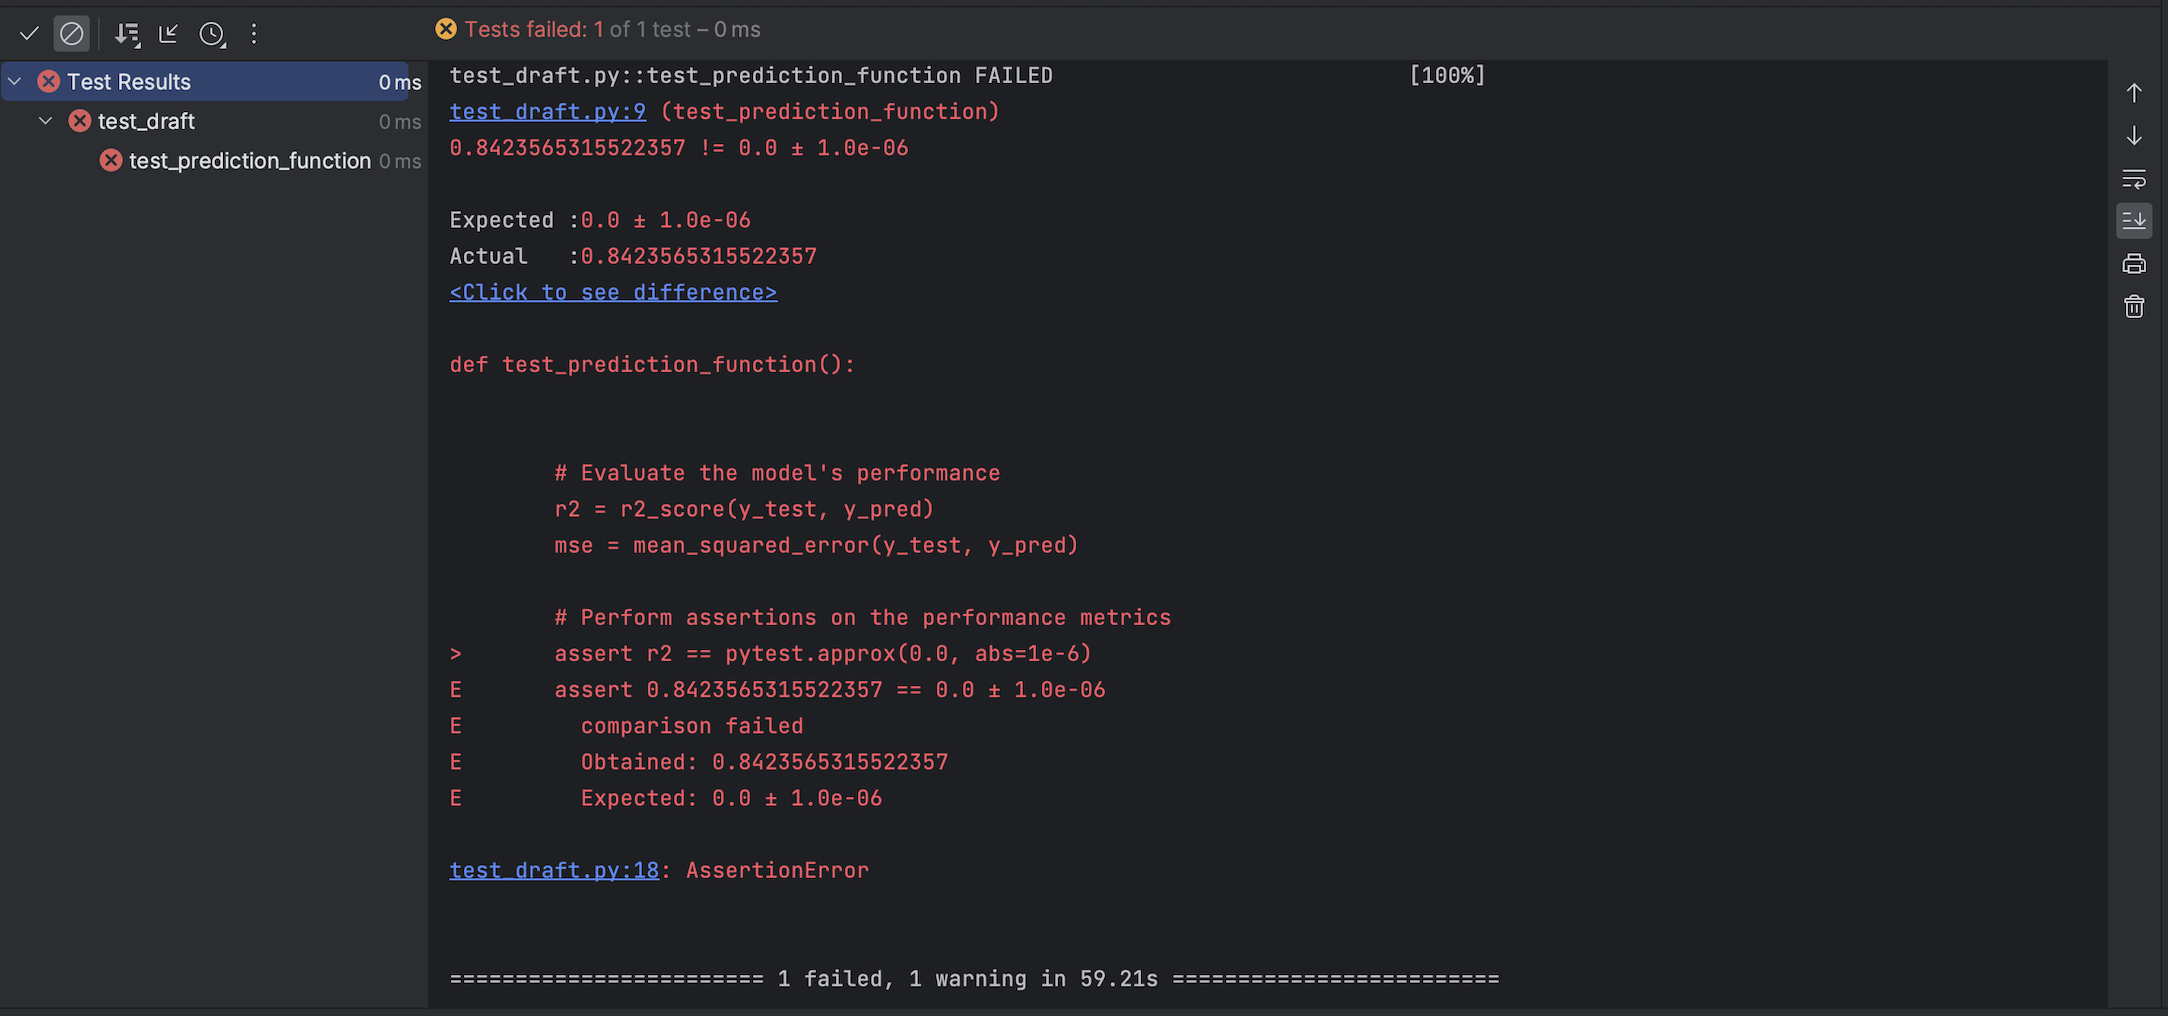
\includegraphics[height=125mm, width=130mm]{Images/TestPred}
					\end{center}
					\caption{ Possible Error for Test Prediction Function }
				\end{figure}
			\end{center}
		
		\end{enumerate}
	
	
	\section{FlowChart}
	
	\begin{center}
		\begin{figure}[h!]
			\begin{center}
				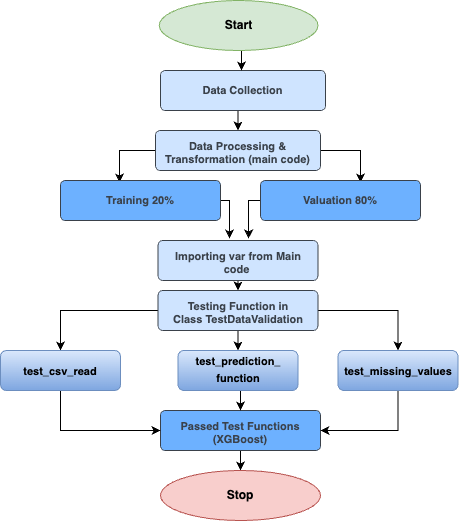
\includegraphics[height=125mm, width=130mm]{Images/TestFunFlowChart}
			\end{center}
			\caption{ FlowChart for Testing Functions }
		\end{figure}
	\end{center}